\chapter[Mixing Properties of Individual Enrichment Sources as a Function of Energy]{Mixing Properties of Individual Enrichment Sources as a Function of Energy\label{ch:chapter4}}
\let\thefootnote\relax\footnotetext{This section contains unpublished work-in-progress}

%
% Copy paste paper here, without abstract or keywords
%

\section{Introduction}

\section*{Acknowledgments}

\section{Methods}
\label{ch4:sec:methods}
We refer the reader to the previous chapters for more detailed descriptions of our numerical methods and feedback models. The mixing experiments discussed below are conducted in restarted versions of the same low-mass, isolated galaxy simulations used throughout this work.


%We refer the reader to Paper I for a detailed description of our numerical methods and feedback models. We briefly summarize the relevant details here.

% Summarize details here for the paper, but I'm not sure if its needed for the thesis chapter.

\subsection{Mixing Experiment Setup}
\label{ch4:sec:experiment}
We restart our fiducial, full-physics simulation at three different times, 100 Myr, 180 Myr, and 360 Myr; runs at these times are labelled as I, II, and III respectively. These correspond to three different times in the galaxy's SFR evolution, testing how much variance is expected in the metal mixing and ejection with the star formation rate. I occurs in the last $\sim$ 20 Myr of the initial burst of star formation, II occur during the lull in star formation following this peak, and III in an extended period of little to no ongoing star formation. We attempted to to evolve each simulation for 150 Myr, but due to computational constrains (particularly with the I runs) this was not always possible.

At the beginning of each restart, we place by-hand one or more enrichment events at assigned positions throughout the galaxy, with thermal injection energies ($E_{\rm ej}$), masses ($m_{\rm ej}$), and metal fractions ($Z_{\rm ej}$). We note that the injection masses, particularly the metal fractions, are somewhat arbitrary as they are likely dynamically insignificant relative to the ambient ISM mass in which they occur. The important parameter here is $E_{\rm ej}$, which we vary to sample the range of ejection energies associated with significant sources of chemical enrichment, including AGB winds ($10^{46}$~erg)\footnote{Assuming full thermalization of the total mechanical energy output of an AGB wind.}, NS-NS mergers ($10^{49} - 10^{50}$~erg), supernovae (10$^{51}$~erg), and exotic enrichment sources, such as hypernovae, that can reach much higher energies (10$^{52}$~erg). Each run contains only sources from a single event type, as indicated in the run-name by the log of the injection energy in ergs. For example, the run beginning at 180~Myr with AGB-like events is labeled ``II\_E46". The metal enrichment from each source is tracked and evolved with a unique passive scalar tied to the individual source and separate from any additional chemical enrichment that may occur within the galaxy over time.

Each run contains multiple events spread over the galaxy to test how radial and azimuthal position in the galaxy affects mixing and ejection, but limited to ensure that the events do not overlap and influence each other dynamically. For the low-energy events, we are able to run 19 events per restart, while the $10^{49}-10^{51}$~erg runs contain 7 events, and the 10$^{52}$~erg runs only contain a single event.

Most of this analysis refers to these average behavior of the metals from these enrichment events over time as a way to gain a general appreciation for how $E_{\rm ej}$ and galactic properties affect the evolution of metals. However, we do note that this is not fair statistically, as the higher energy runs are undersampled.

%We discuss how radial and azimuthal position affects the evolution in


\section{Results}

Perhaps the three most important parameters to quantify for each enrichment event are: 1) what fraction of released metals are immediately available for star formation, 2) what fraction of metals are carried out of the galaxy in outflows, and 3) how and over what timescale do metals cool from hot phases into star forming gas. We discuss each of these points in Section~\ref{ch4:sec:ISM CGM}. In Section~\ref{ch4:sec:spreads} we go further and address the relative homogeneity of the metals retained by the ISM for each enrichment source.

We focus this analysis primarily on the results from run II, and save a discussion of how these results vary across runs and across specific source positions in Section XXX \textit{(maybe take out if don't have time)}.

\subsection{Enrichment of the ISM and CGM}
\label{ch4:sec:ISM CGM}

We summarize the source-averaged results for all enrichment events in runs II\_E46, II\_E49, II\_E50, II\_E51, and II\_E52 in Figure~\ref{ch4:fig:ISM_CGM} by showing the fraction of source metals contained within each phase of the ISM (colored lines, which sum to the black dashed line), and the CGM (black, solid). These plots show a clear, immediate trend across $E_{\rm ej}$ for all lines in the figure, but the differences are most striking for the ISM (black, solid), CGM (black, dashed) lines. In Chapter~\ref{ch:chapter3}
% \citep{Emerick2019}
we demonstrated that there was a significant difference in metal ejection fraction, $f_{\rm ej}$, for metals from AGB sources as compared to metals released in SNe. Here, we confirm that this is driven predominantly by differences in the energy of the events, and not necessarily when or where they occur in the ISM. The clear trend in Figure~\ref{ch4:fig:ISM_CGM} shows that events with higher $E_{\rm ej}$ are much more readily ejected from the disk of the galaxy, while events with lower $E_{\rm ej}$ couple poorly to the same galactic outflows.
\textit{statement on how immediate enrichement is after events}
% By 10~Myr after the enrichment events,
The high-energy events rapidly converge on a peak $f_{\rm ej}$ within about 20~Myr of the event, with only a gradual increase towards the end of the 150~Myr as the metals in the ISM are swept up in additional outflows. The lower energy events evolve more gradually. The lowest energy event, corresponding to AGB winds, reaches $f_{\rm ej}$ ~ 0.68, which increases to 0.87 for the 10$^{51}$~erg events, and 0.95 for the 10$^{52}$~erg event. This implies that, if one to were assume that all metals behaved the same and adopted an $f_{\rm ej}$ of $\sim$0.9, typical of SNe-like events (and which is comparable to that observed for O in Local Group dwarf galaxies, \citep{Kirby2011,McQuinn2015}), one would underestimate the amount of AGB metals in the ISM by a factor of $\sim$ 3, and overestimate exotic, high-energy sources by a factor of $\sim$2.
% This ejection fraction is a critical ingredient in chemical evolution models, and the fact that it varies with enrichment source can


\begin{figure*}
\centering
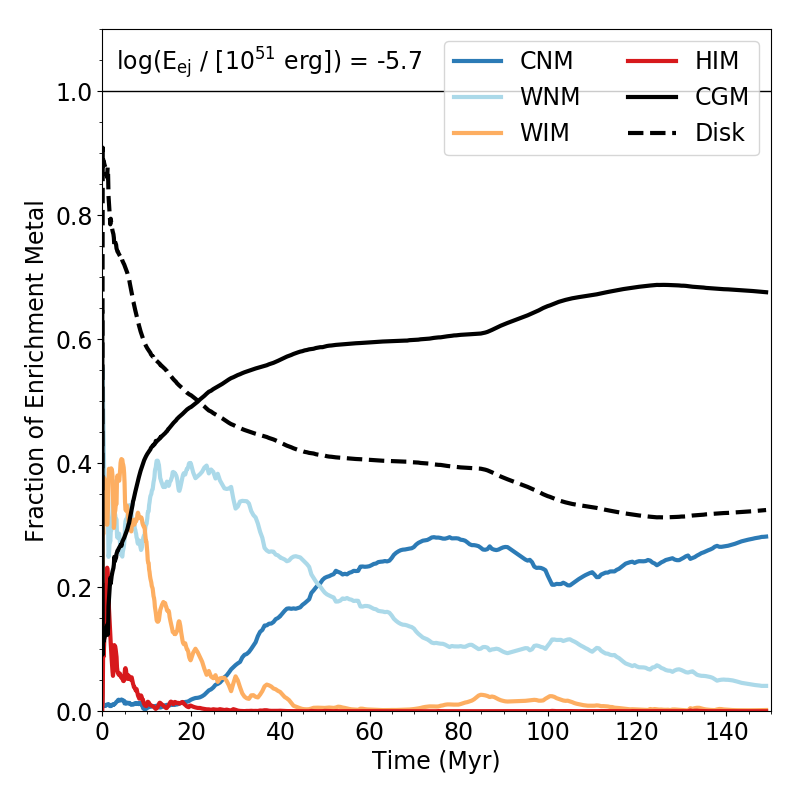
\includegraphics[width=0.45\linewidth]{figures/ch4/AGB1_enrichment_evolution_average_CGM}
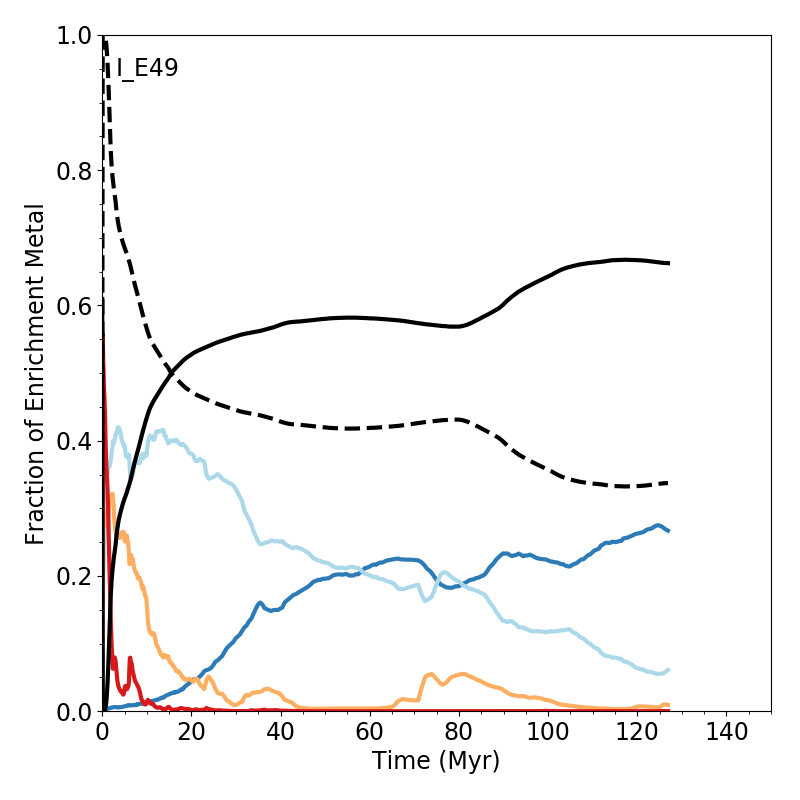
\includegraphics[width=0.45\linewidth]{figures/ch4/NSNS1_enrichment_evolution_average_CGM} \\
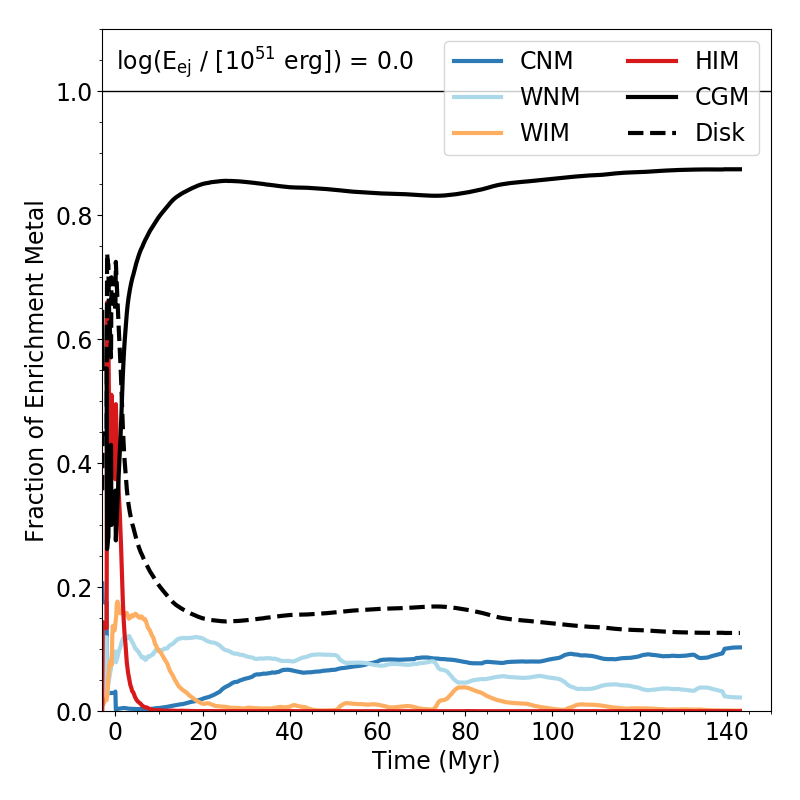
\includegraphics[width=0.45\linewidth]{figures/ch4/SNE1_enrichment_evolution_average_CGM}
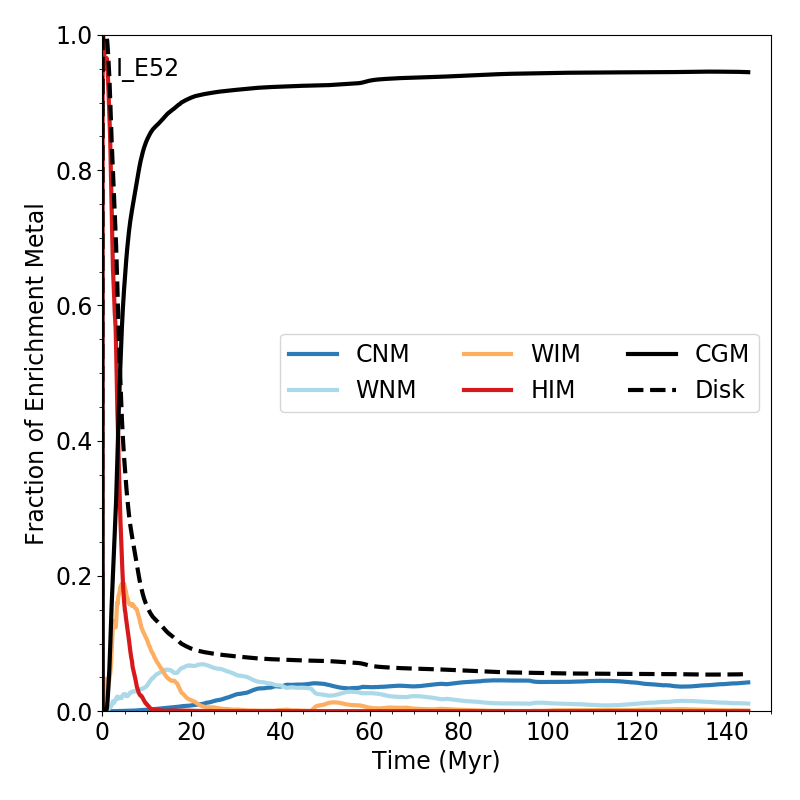
\includegraphics[width=0.45\linewidth]{figures/ch4/HNE1_enrichment_evolution_average_CGM}
\caption{Time evolution of the }
\label{fig:ch4:ISM_CGM}
\end{figure*}


% make a figure here showing JUST the CNM evolution of the ISM for each source

\subsection{Homogeneity of Mixing}
\label{ch4:sec:spreads}

%************* APPENDICES ************************%

%\clearpage
%\appendix - Liklely DO NOT use this command
\setcounter{section}{0}%
\renewcommand\thesection{\thechapter.\Alph{section}}

%
% Place appendix here
%

\renewcommand\thesection{\thechapter.\arabic{section}}
